\subsection{First Current Mirror Circuit}
% Current mirror 1
\FloatBarrier

\begin{figure}[h!]
	\centering
	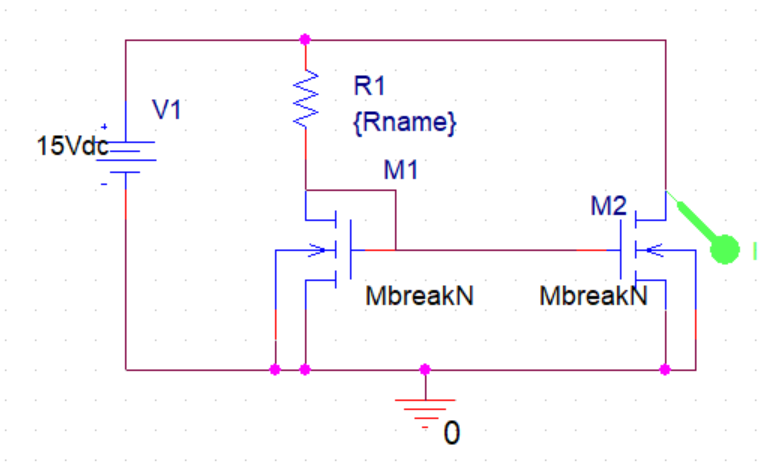
\includegraphics[scale=0.75]{./images/circuit4.PNG}
	\caption{First Current Mirror Circuit}
	\label{fig:circuit4}
\end{figure}

\FloatBarrier

% How the current mirror works
Assume transistors $M_1$ and $M_2$ in figure (\ref{fig:circuit4}) are identical. Because $M_1$ is a diode-connected MOSFET, if $V_{DS} = V_{GS} > V_T$, then $M_1$ operates in saturation. Assume that $M_1$ is not in cutoff and is therefore in saturation. $M_1$'s drain current shall be called $i_{ref}$, and $M_2$'s $i_{out}$. \\

Because the gates of $M_1$ and $M_2$ are connected and both of their sources are grounded, $V_{GS}$ is the same for each. Since $M_1$ and $M_2$ are identical transistors, their $V_{T}$ values are identical as well. So, if current can flow through $M_1$'s drain, then $M_2$ must also be active because $V_{GS} > V_{T}$ in both cases. $M_2$'s $V_{DS}$ certainly exceeds $M_1$'s $V_{DS}$ since $M_2$'s drain is directly connected to the supply voltage rather than an intermediary resistor. Since $M_1$ is in saturation, $V_{DS} > V_{GS} - V_{T}$ is the condition for saturation, and $M_2$'s $V_{DS}$ exceeds $M_1$'s $V_{DS}$, then $M_2$ must also be in saturation. \\

Since both transistors are in saturation, have the same $V_{GS}$ value, and have identical structures, the following must be true:

\begin{equation}
	\label{eq:current_mirror_eqn}
	\frac{ i_{ref} }{ i_{out} } = \frac{ \frac{k_n}{2} ( V_{GS} - V_{T} )^2 }{ \frac{k_n}{2} ( V_{GS} - V_{T} )^2 } = 1 \rightarrow i_{ref} = i_{out}
\end{equation}

This circuit is called a "current mirror" because of the property demonstrated in equation (\ref{eq:current_mirror_eqn}). Given any input current $i_{ref}$, the output current $i_{out}$ must be the same. Changing the dimensions of the transistors relative to one another can alter the output current by a constant factor \cite{current_src_dim}. \\

\FloatBarrier

\begin{figure}[h!]
	\centering
	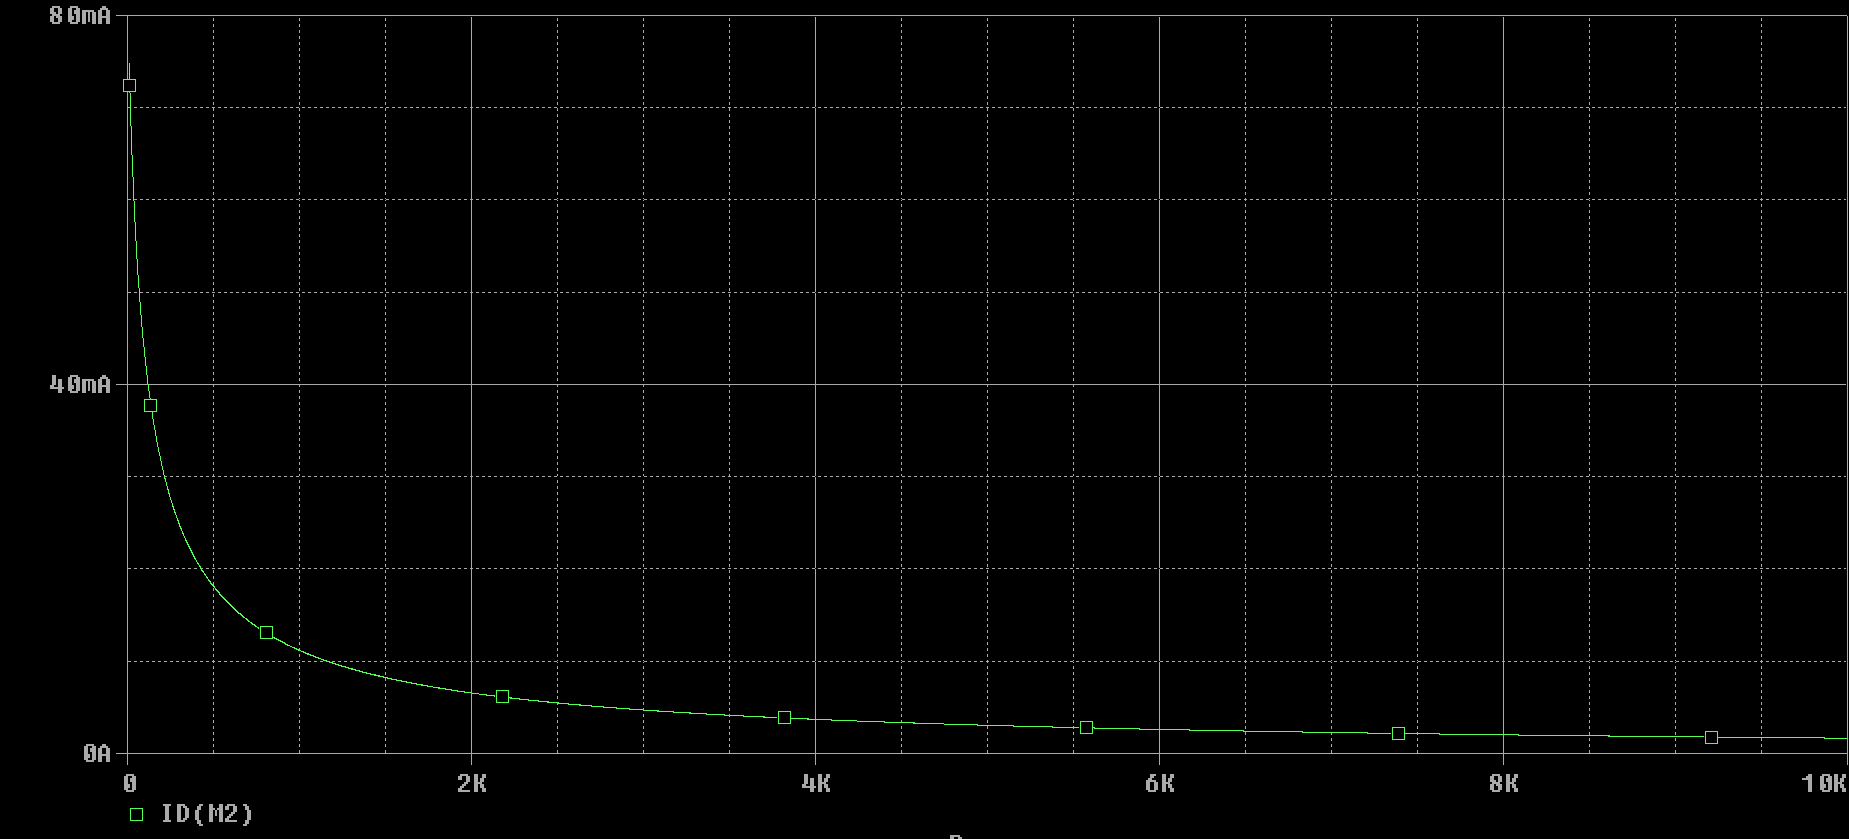
\includegraphics[scale=0.5]{./images/circuit4_r_sweep.PNG}
	\caption{$i_{out}$ versus $R_1$ for Current Mirror in Figure (\ref{fig:circuit4})}
	\label{fig:circuit4_r_sweep}
\end{figure}

\FloatBarrier

In the extreme case where $R_1$ is a short and $V_{T} < V_{DD}$ (as it should be), where $V_{DD}$ is the supply voltage, then $V_{GS} = V_{DD} > V_{T}$. Thus, $M_1$ and therefore $M_2$ are both in the saturation region. At this point, $V_{GS}$ is maximum, and the maximum $i_D$ should flow. \\

On the other hand, if $R_1$ is an open circuit, current cannot flow through $M_1$'s drain. Furthermore, current cannot flow from $M_1$'s gate to its drain because it would need to be supplied by current from one of the transistors' gates. Therefore, $M_1$ cannot receive any drain current. So, as $R_1 \rightarrow \infty$, $i_D = 0$. Thus, as $R_1$ is increased, it absorbs more and more of the supply voltage $V_{DD}$ until $M_1$ operates in cutoff mode. Thus, the $i_{ref}$ versus $R_1$ curve should be downward sloping. \\

\subsection{Second Current Mirror Circuit}
% Current mirror 2

\FloatBarrier

\begin{figure}[h!]
	\centering
	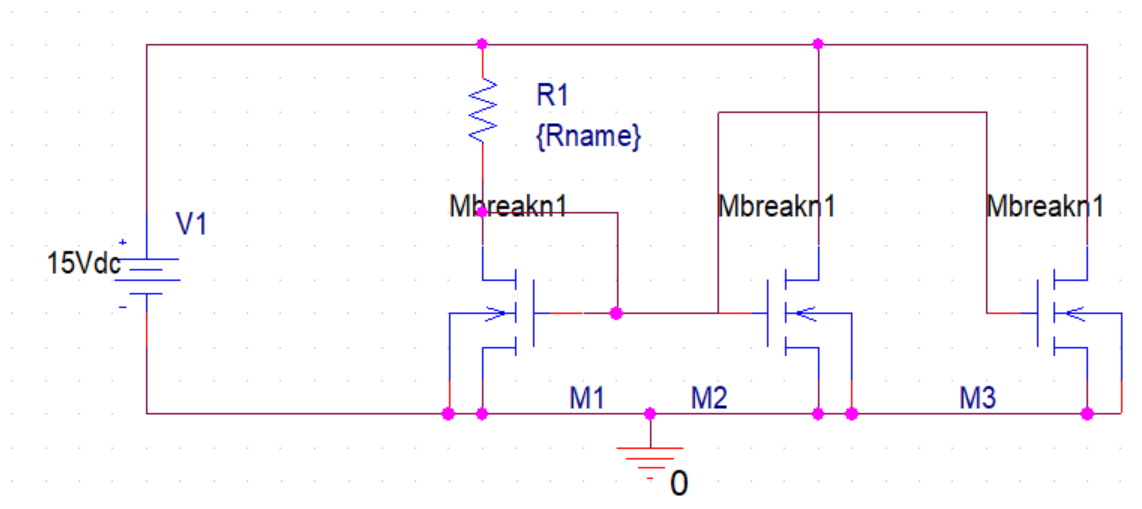
\includegraphics[scale=0.75]{./images/circuit5.PNG}
	\caption{Second Current Mirror Circuit}
	\label{fig:circuit5}
\end{figure}

\FloatBarrier

The circuit in figure (\ref{fig:circuit5}) is simply an extension of the circuit in figure (\ref{fig:circuit4}). By the same physical principles described earlier, the currents through $M_2$ and $M_3$ should be individually identical to the current $i_{ref}$ running through $M_1$. The $i_D$ versus $R_1$ curve should be essentially the same as the one in the previous circuit since the physical situation (voltages at each node of $M_1$) should be the same.

\FloatBarrier

\begin{figure}[h!]
	\centering
	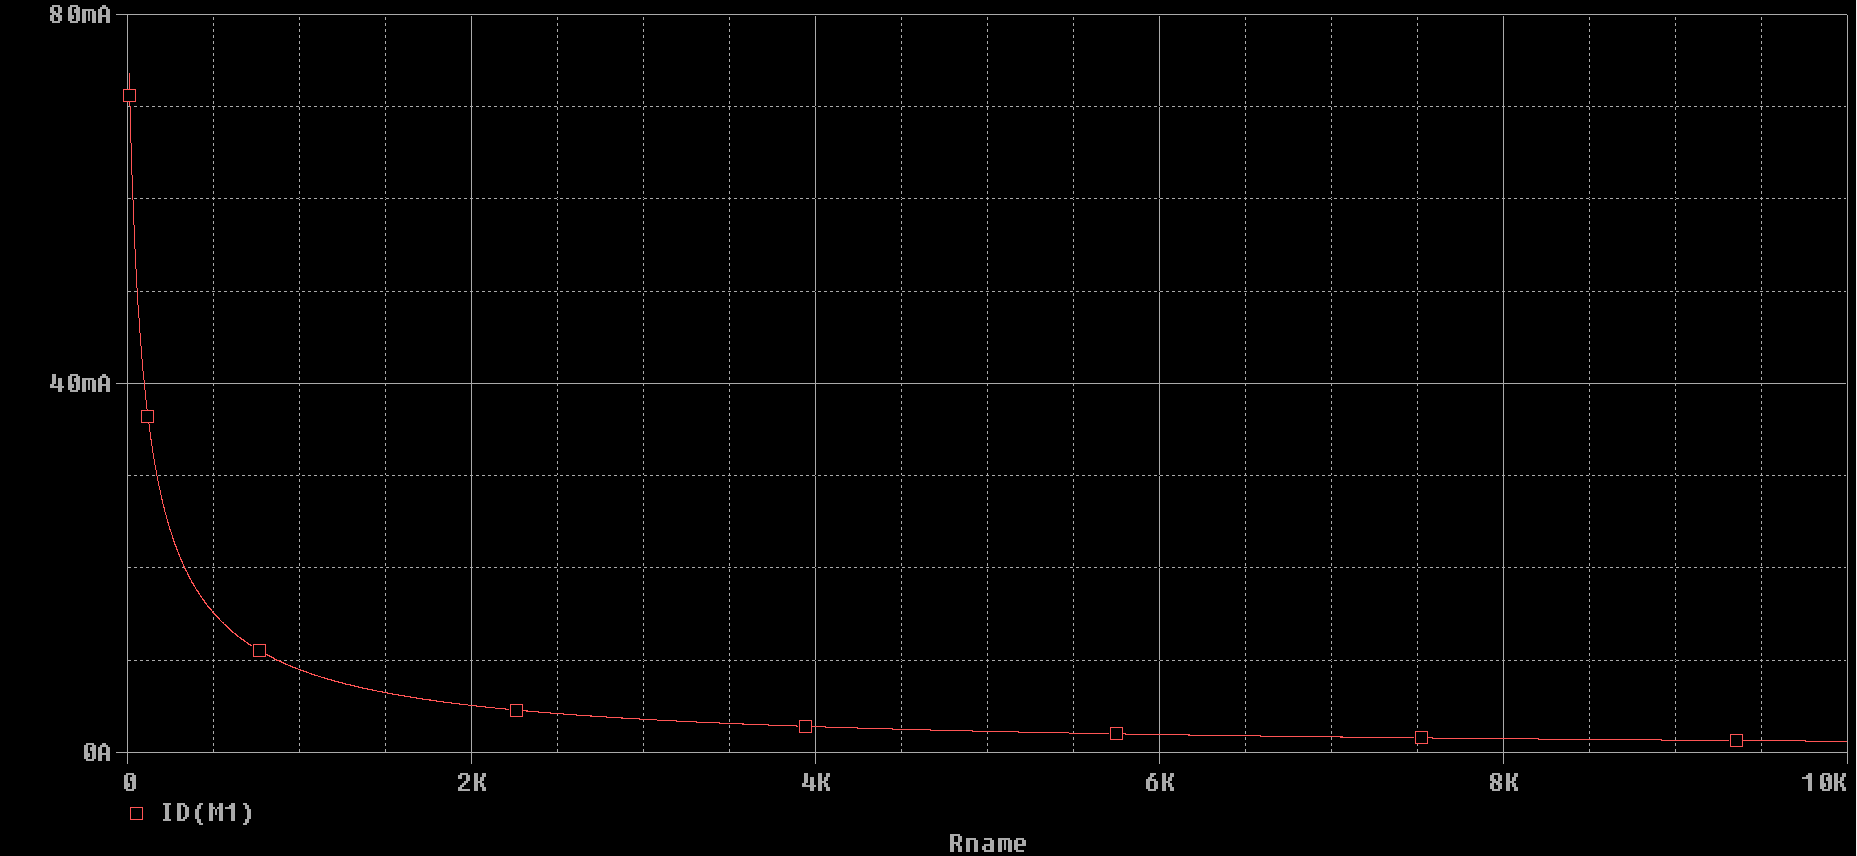
\includegraphics[scale=0.5]{./images/circuit5_r_sweep.PNG}
	\caption{$i_{D,M1}$ versus $R_1$}
	\label{fig:circuit5_id1_vs_r}
\end{figure}

\FloatBarrier

Since the currents through $M_2$ and $M_3$ should each be $i_{ref}$, their sum should be about $2i_{ref}$. For instance, at $R_1 = 10$\si{\ohm}, $i_{ref}$ from figure (\ref{fig:circuit5_id1_vs_r}) is about $75$\si{\milli\ampere}. The sum of the currents in figure (\ref{fig:circuit5_id2_plus_id3_vs_r}) is about $150$\si{\milli\ampere}, twice that value. The curve follows the same trend, but with double the values for this reason.

\FloatBarrier

\begin{figure}[h!]
	\centering
	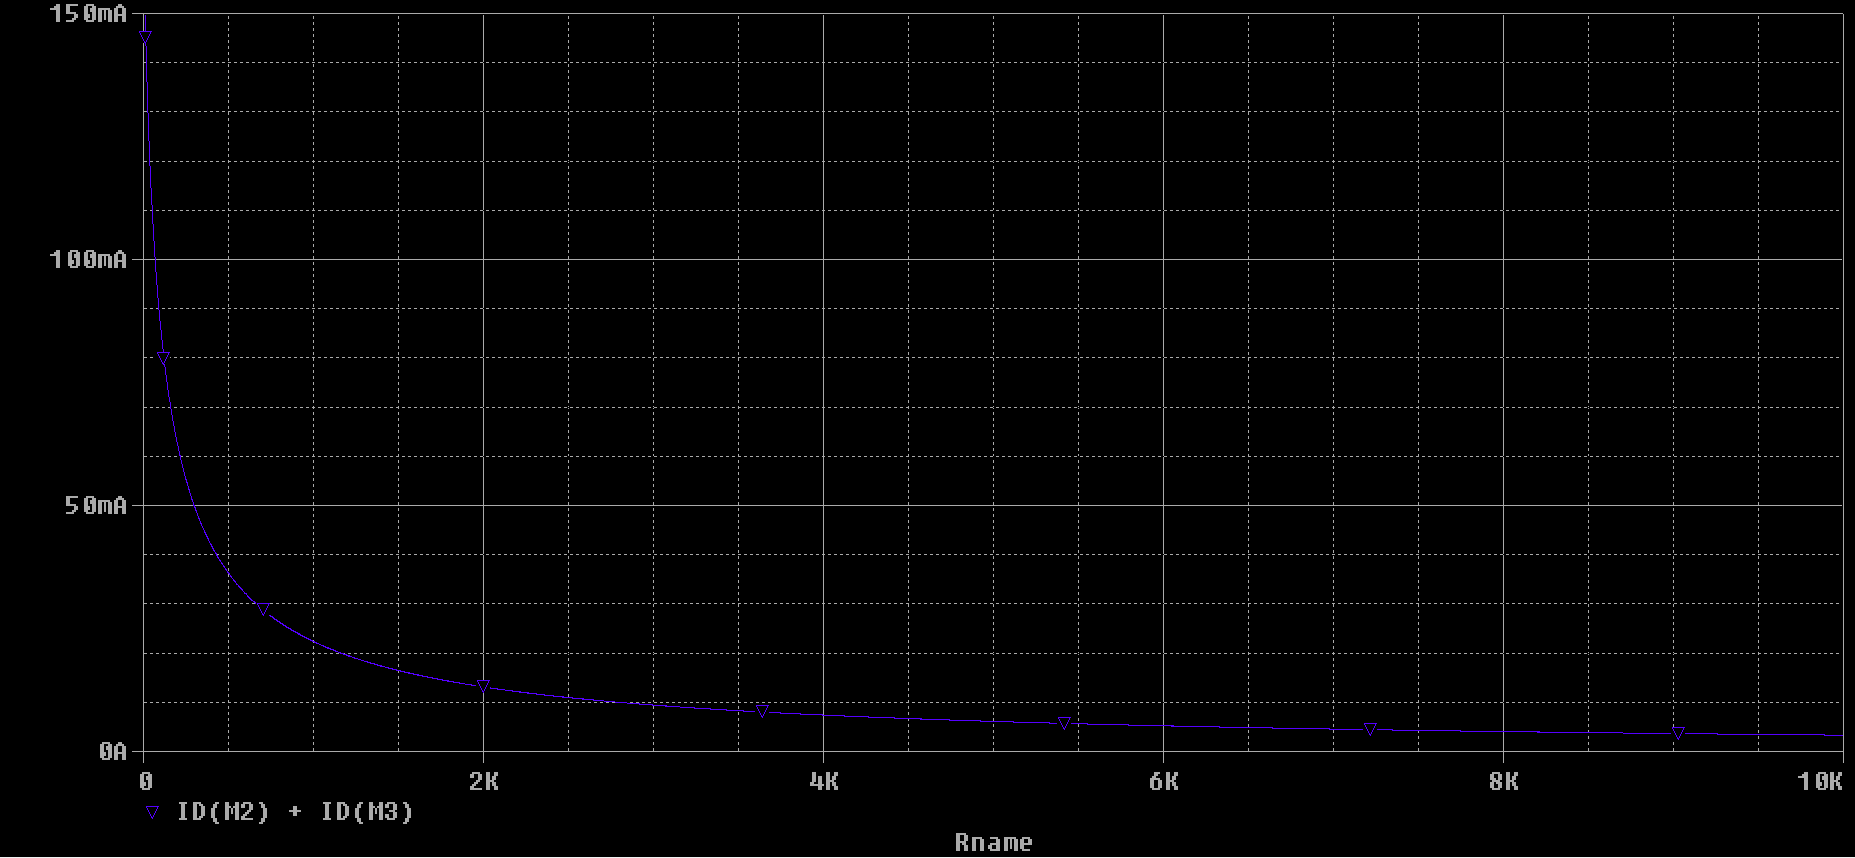
\includegraphics[scale=0.5]{./images/circuit5_sum_r_sweep.PNG}
	\caption{$i_{D,M2} + i_{D,M3}$ versus $R_1$}
	\label{fig:circuit5_id2_plus_id3_vs_r}
\end{figure}

\FloatBarrier
